\subsection{Results}
\label{sec:results}

In this section, we systematically evaluate the generative performance of the proposed network models by comparing the simulated social contact patterns against the empirical POLYMOD dataset.
The assessment progresses from macroscopic network volume to microscopic, localized age-mixing structures, concluding with a holistic evaluation of the structural residuals.

\subsubsection{Summary Statistics Recovery and Structural Trade-offs}

Before examining the graphical properties of the generated networks, it is essential to verify the behavior of the Simulation-based Inference (SBI) engine.
Table \ref{tab:zscore_recovery} presents a comparison between the empirical target statistics and the posterior predictive distributions for Model 1 and Model 2B.
The accuracy of the parameter recovery is quantitatively assessed using Z-scores.
For Model 1, the highly flexible, generalized architecture allows the MCMC algorithm to perfectly calibrate to the macroscopic targets, resulting in Z-scores close to zero.
In contrast, Model 2B reveals a more nuanced, highly informative dynamic.
The strict, deterministic boundaries introduced to capture school cohorts successfully recovered their localized targets, with the proportions for Primary, Secondary, and Tertiary contacts all falling well within the acceptable $|Z| \le 2.0$ threshold.
However, this localized precision introduces a necessary bias-variance trade-off within the generative architecture.
By strictly constraining the model to reproduce rigid, step-like educational structures, the model sacrifices some degrees of freedom required to capture the extreme tails of the global degree distribution (e.g., the underestimation of super-spreaders, indicated by the large Z-score for $\text{Prop Degree} \ge 25$).
This discrepancy is not a failure of the inference, but rather a fundamental characteristic of highly stratified network models: enforcing strict local homophily inevitably restricts global distributional flexibility.
Having confirmed that the underlying structural rules were successfully extracted by the inference engine, the subsequent sections visually and quantitatively dissect how these localized rules manifest across the entire contact network.

\begin{table}[H]
    \centering
    \caption{Posterior predictive checks (Z-scores) for selected summary statistics. While Model 1 seamlessly fits broad macroscopic targets, Model 2B demonstrates a trade-off: it successfully captures rigid local structures (school cohorts) at the expense of extreme distributional tails.}
    \label{tab:zscore_recovery}
    \begin{tabular}{lccc}
        \toprule
        \textbf{Statistic} & \textbf{Empirical Target} & \textbf{Simulated Mean} & \textbf{Z-Score} \\
        \midrule
        \multicolumn{4}{l}{\textit{Panel A: Model 1 Targets}} \\
        Mean Degree & 13.53 & 13.67 & -0.13 \\
        Log Variance & 4.72 & 4.75 & -0.13 \\
        Mean Age Difference & 15.17 & 15.16 & 0.03 \\
        Proportion MM & 0.26 & 0.26 & 0.06 \\
        Proportion FF & 0.30 & 0.31 & -0.10 \\
        \midrule
        \multicolumn{4}{l}{\textit{Panel B: Model 2B Targets (Selected)}} \\
        Log Mean Degree & 2.61 & 2.59 & 1.90 \\
        Proportion Age 6--15 & 0.186 & 0.184 & 0.81 \\
        Proportion Primary Low & 0.028 & 0.025 & 1.65 \\
        Proportion Secondary & 0.097 & 0.102 & -1.46 \\
        Proportion Tertiary & 0.031 & 0.032 & -0.37 \\
        Proportion Degree $\ge 25$ & 0.148 & 0.123 & 11.26 \\
        \bottomrule
    \end{tabular}
\end{table}

\subsubsection{Macroscopic Network Volume and Degree Distribution}

The most fundamental characteristic of a contact network is its overall volume and the distribution of connections among individuals.
Figure \ref{fig:mean_degree} illustrates the mean total contacts across different age groups.
The empirical POLYMOD data reveals a distinct peak in contact volume among school-aged children and young adults, followed by a gradual decline in older populations.
Model 1, constrained by a uniform baseline density parameter, systematically underestimates the contact volume for younger cohorts and overestimates it for the elderly, resulting in a relatively flat degree profile.
In contrast, both Model 2A and Model 2B successfully reproduce the elevated contact rates among youths.
This improvement is directly driven by the integration of targeted educational attributes.

\begin{figure}[H]
    \centering
    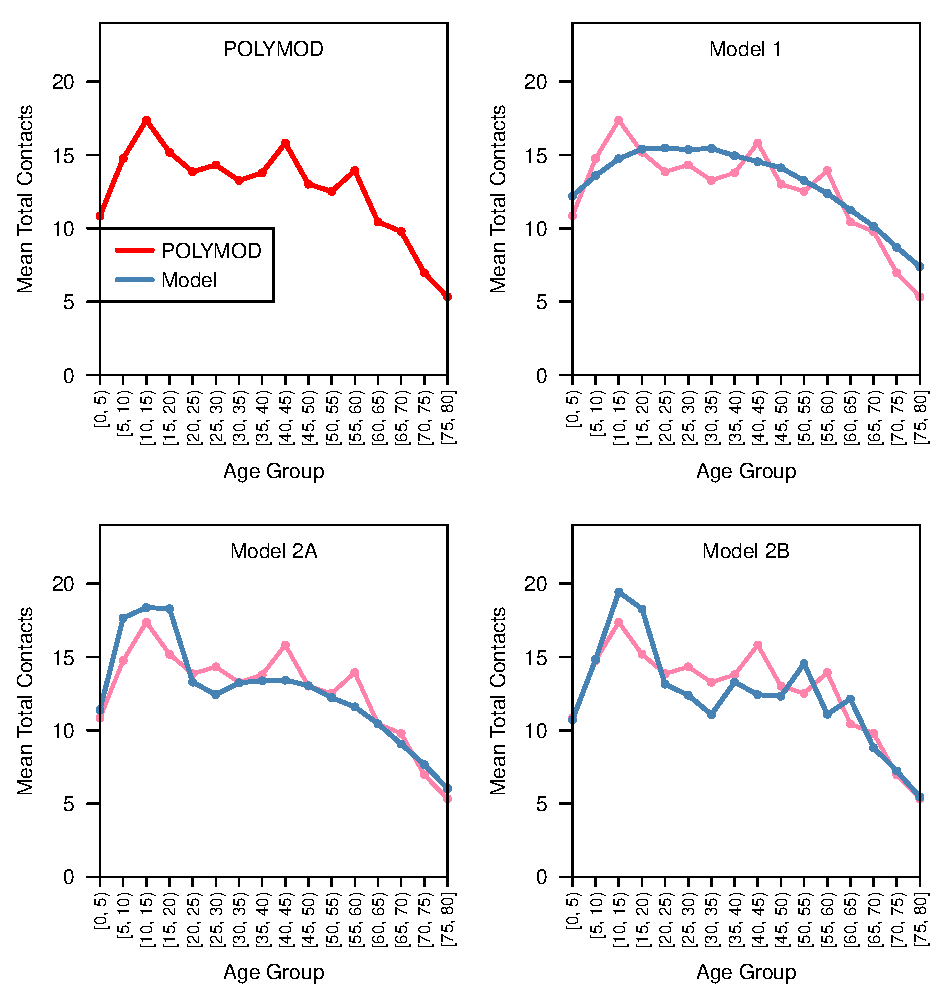
\includegraphics[width = 0.85\linewidth]{figures/03_NetworkModel/mean_degree_2x2.pdf}
    \caption{Comparison of mean total contacts (degree) by age group. Model 2 architectures successfully capture the elevated contact rates among younger populations compared to the flat profile of Model 1.}
    \label{fig:mean_degree}
\end{figure}

Beyond the mean values, examining the Cumulative Distribution Function (CDF) of the degree (Figure \ref{fig:degree_cdf}) provides critical insights into the dispersion of sociability.
Empirical contact networks are typically characterized by overdispersion, where a small fraction of highly sociable individuals acts as super-spreaders.
All three models effectively capture the broad shape of the empirical CDF.
This confirms that the individual-level random effect for sociability ($\epsilon_i$), introduced in the foundational equation, successfully models the variance and long-tail behavior of human interactions across all proposed architectures.

\begin{figure}[H]
    \centering
    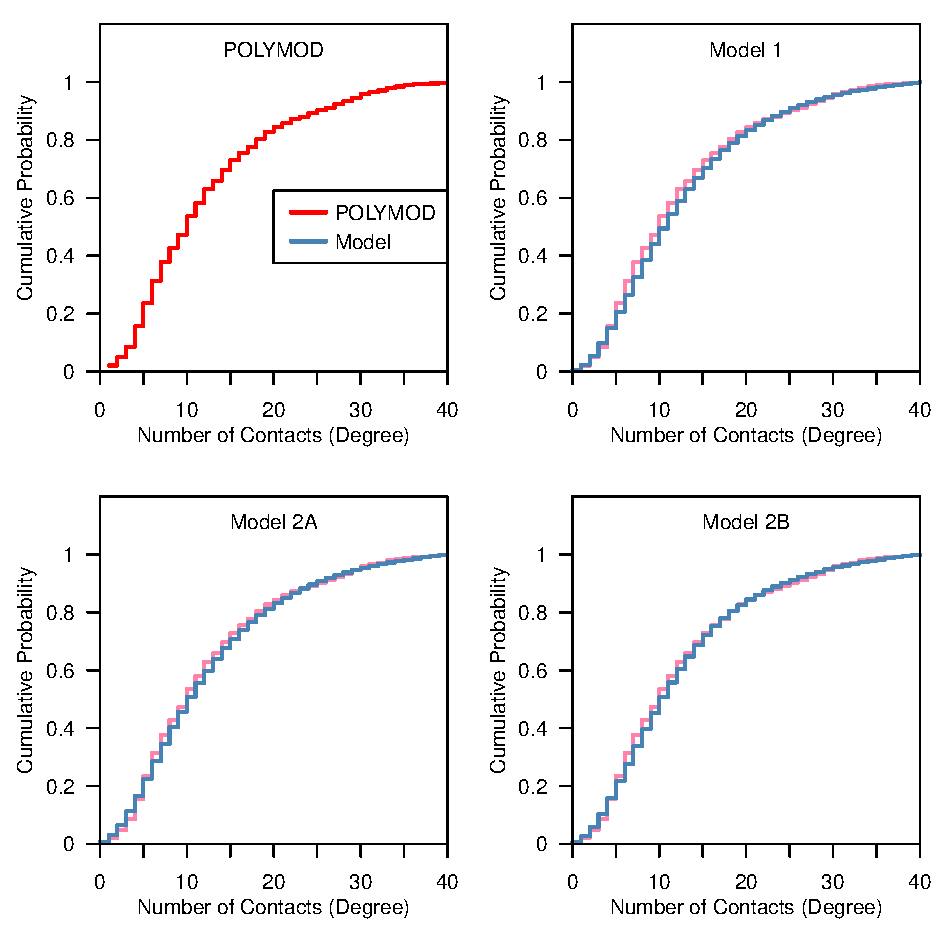
\includegraphics[width = 0.85\linewidth]{figures/03_NetworkModel/degree_cdf_2x2.pdf}
    \caption{Cumulative Distribution Function (CDF) of the number of contacts (degree). The node-specific random effects successfully capture the overdispersion and super-spreader tails across all models.}
    \label{fig:degree_cdf}
\end{figure}

\subsubsection{Meso-structure: Age Mixing Mechanisms}

While macroscopic metrics describe the overall volume of contacts, they do not capture the specific topological patterns of who interacts with whom.
Figure \ref{fig:agediff_dist} displays the probability distribution of absolute age differences between interacting individuals.
The empirical POLYMOD data exhibits a distinct bimodal characteristic: a sharp, exponentially decaying peak at an age difference of zero, representing intra-generational (peer) interactions, and a wider, normally distributed bump around 20 to 35 years, reflecting inter-generational (household) interactions.
Model 1 relies on a single continuous logit-linear function for age difference, resulting in a monotonically decreasing probability that completely fails to capture the inter-generational household bump.
By introducing a mixture distribution approach, both Model 2A and Model 2B successfully reproduce this complex bimodal mechanism.
They accurately generate both the sharp peer-to-peer spike and the broader parent-child mixing patterns.
This bimodal capture is further supported by the CDF of age differences shown in Figure \ref{fig:agediff_cdf}, where Model 2 architectures perfectly align with the empirical curve.

\begin{figure}[H]
    \centering
    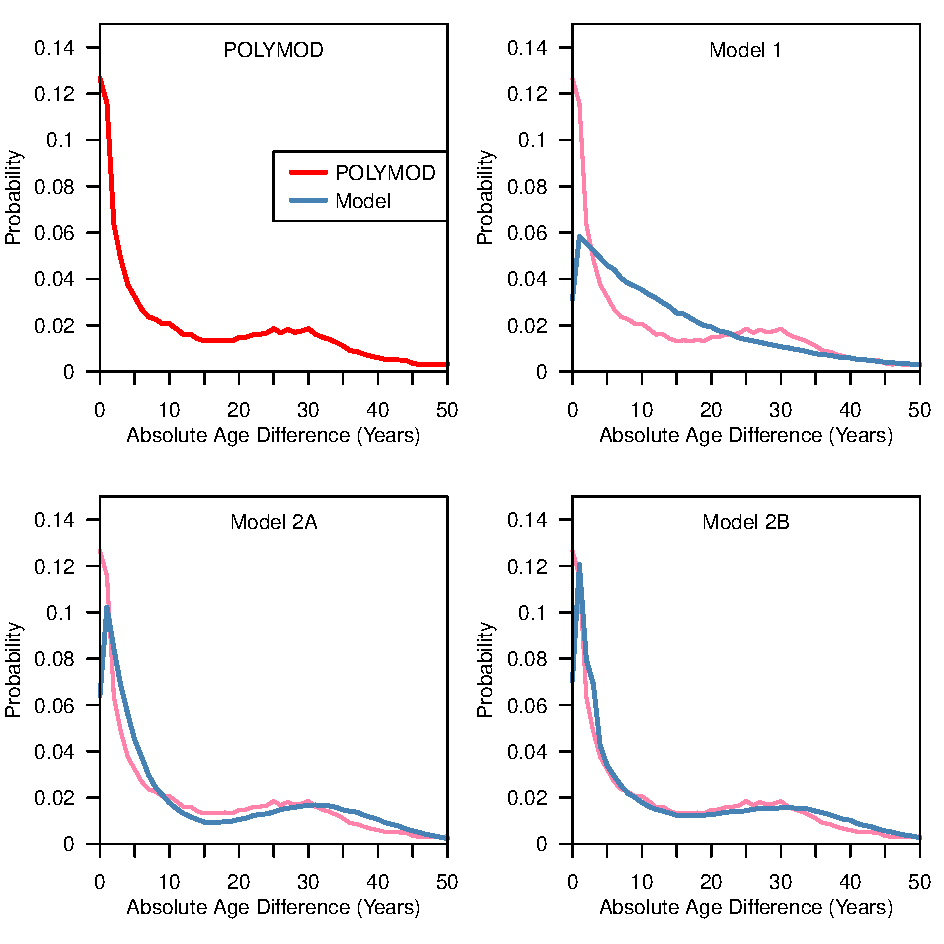
\includegraphics[width = 0.85\linewidth]{figures/03_NetworkModel/agediff_dist_2x2.pdf}
    \caption{Probability distribution of absolute age differences between contacting pairs. The mixture distribution in Model 2 successfully captures the bimodal nature of peer and household mixing.}
    \label{fig:agediff_dist}
\end{figure}

\begin{figure}[H]
    \centering
    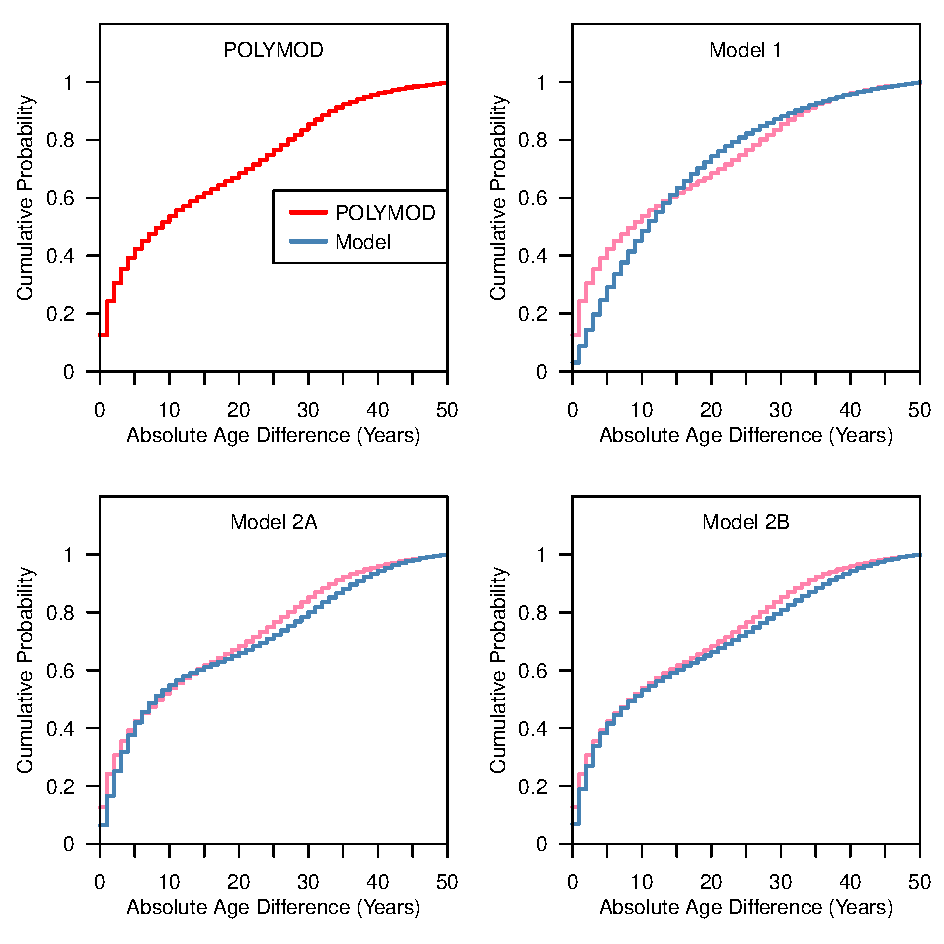
\includegraphics[width = 0.85\linewidth]{figures/03_NetworkModel/agediff_cdf_2x2.pdf}
    \caption{Cumulative Distribution Function (CDF) of absolute age differences, confirming the structural fit of the mixture distribution introduced in the Model 2 framework.}
    \label{fig:agediff_cdf}
\end{figure}

\subsubsection{Micro-structure: Localized Educational Homophily}

Although both Model 2A and 2B successfully capture macro-level and meso-level dynamics, their capabilities diverge significantly at the micro-structural level.
Figure \ref{fig:diag_step} isolates the diagonal elements of the contact matrix, representing the mean number of contacts occurring strictly within the same 5-year age cohort.
The empirical data displays a complex, step-like increase in peer contacts throughout childhood and adolescence, peaking dramatically in the $[10, 15)$ and $[15, 20)$ age groups before collapsing in adulthood.
Model 2A attempts to capture this phenomenon by applying a uniform educational homophily boundary across a broad $5 \le A \le 20$ range.
Consequently, Model 2A generates a flat, averaged plateau of peer contacts, failing to replicate the nuanced demographic gradients.
Conversely, Model 2B introduces highly localized, maximum-age-conditioned indicators representing Lower Primary, Upper Primary, Secondary, and Tertiary education.
This strict stratification allows Model 2B to perfectly fit the step-like empirical spikes.
This stark contrast clearly demonstrates that precise institutional boundaries are strictly required to accurately simulate micro-level societal interactions.

\begin{figure}[H]
    \centering
    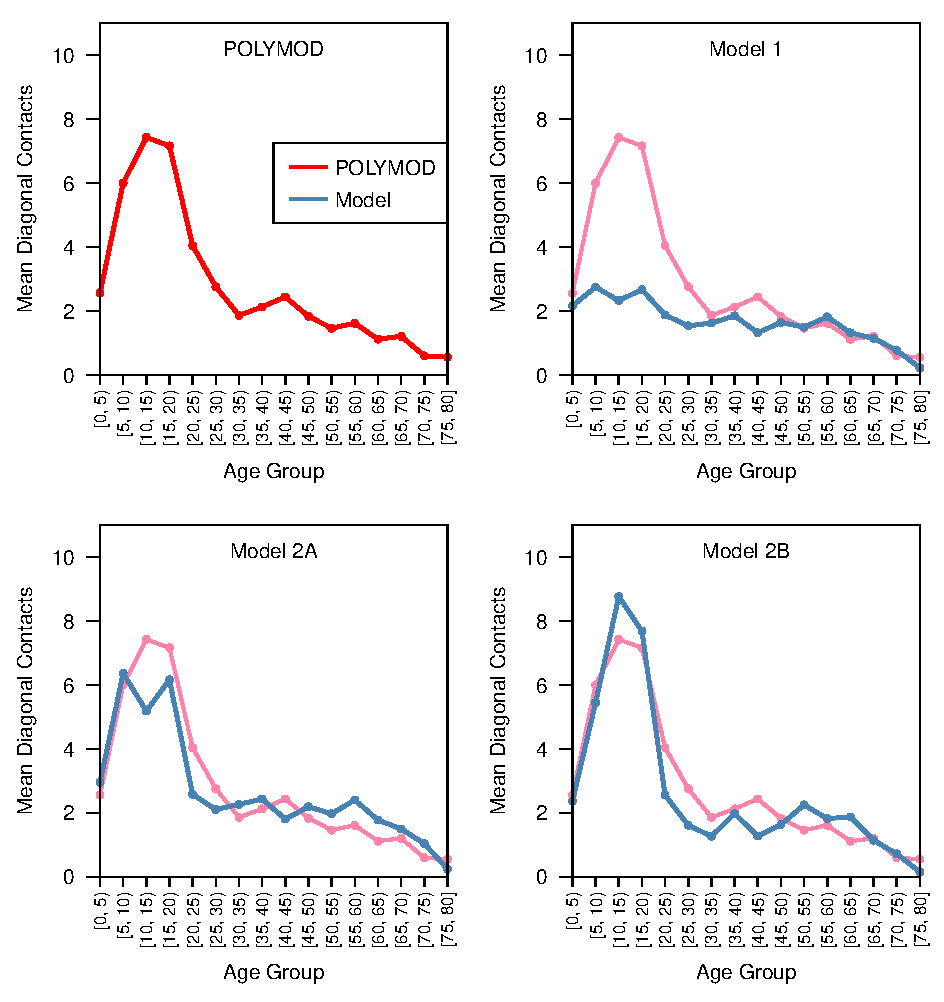
\includegraphics[width = 0.85\linewidth]{figures/03_NetworkModel/diag_step_2x2.pdf}
    \caption{Mean same-age-group (diagonal) contacts across 5-year age brackets. The strictly stratified boundaries in Model 2B are strictly necessary to capture the complex, step-like spikes in school-aged cohorts, exposing the limitations of the homogeneous approach in Model 2A.}
    \label{fig:diag_step}
\end{figure}

\subsubsection{Macro-Synthesis and Error Assessment}

To synthesize the localized micro-structural rules into a holistic perspective, we evaluate the full two-dimensional contact surface.
Figure \ref{fig:contact_matrix} visualizes the simulated contact matrices alongside the empirical POLYMOD matrix, while Figure \ref{fig:residual_matrix} explicitly plots the absolute residuals to highlight areas of systemic bias.
Model 1 exhibits severe, bright red structural residuals, particularly along the diagonal and the sub-diagonal bands, reflecting its inability to model concentrated school and household interactions.
Model 2B, by enforcing the intricate micro-rules discussed in previous sections, systematically neutralizes these systemic errors, resulting in a remarkably clean and white residual map.

\begin{figure}[H]
    \centering
    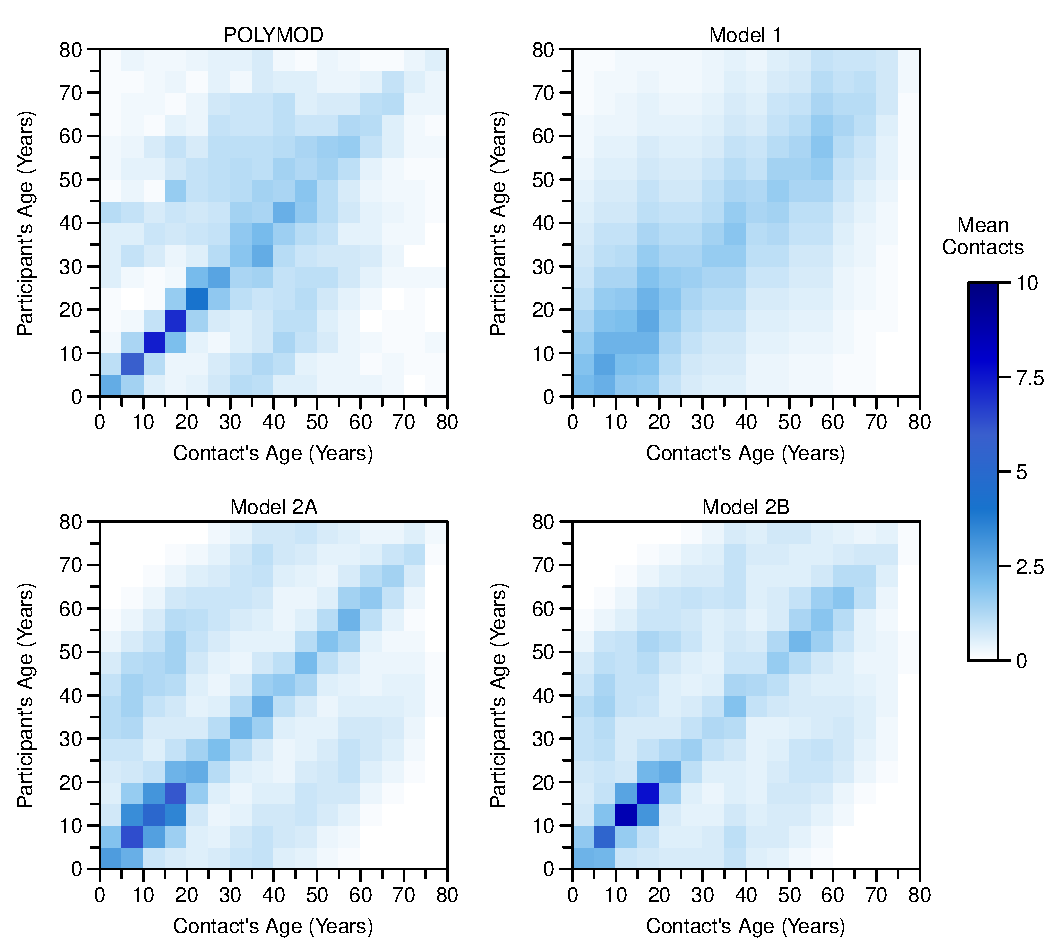
\includegraphics[width = \linewidth]{figures/03_NetworkModel/contact_matrix_2x2_legend.pdf}
    \caption{Two-dimensional contact matrices (heatmaps) comparing the generated networks against the empirical POLYMOD data.
    The intensity of the blue color represents the average number of contacts between individuals in the respective age groups, with more intense colors indicating a higher contact frequency.}
    \label{fig:contact_matrix}
\end{figure}

\begin{figure}[H]
    \centering
    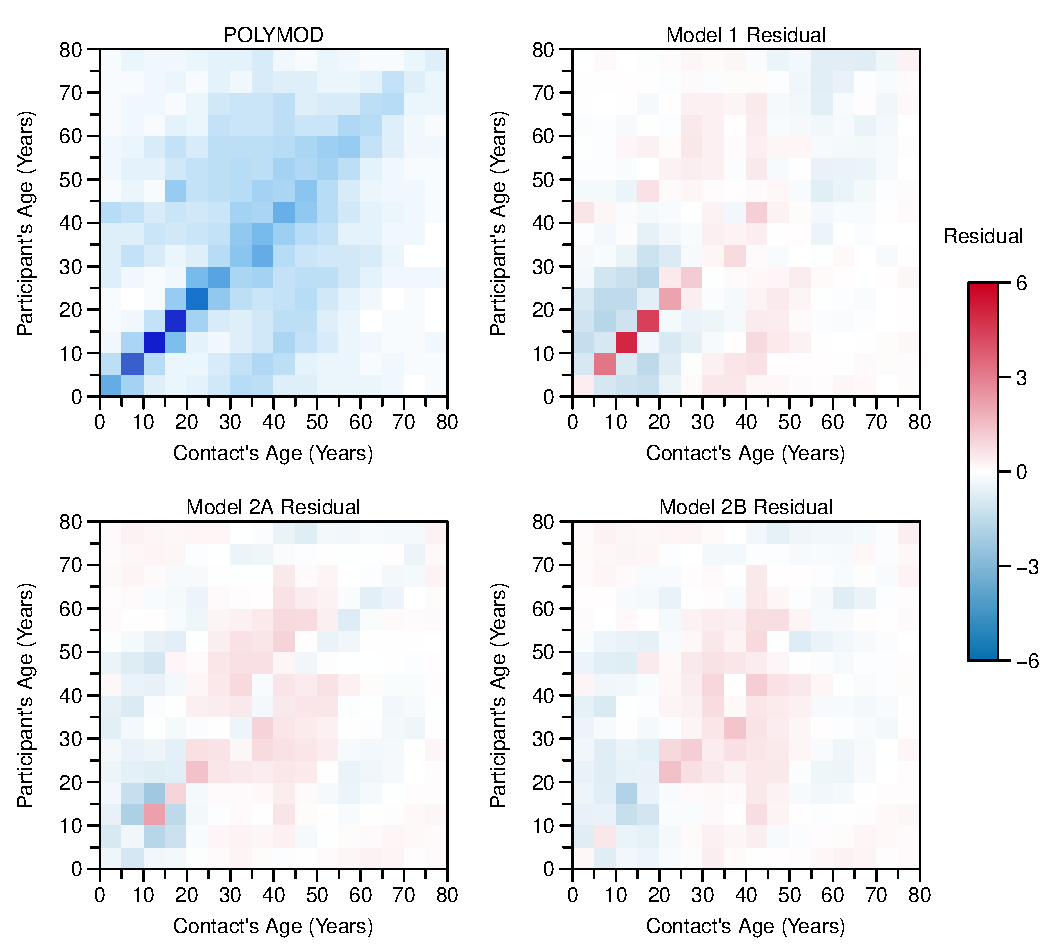
\includegraphics[width = \linewidth]{figures/03_NetworkModel/residual_matrix_2x2_legend.pdf}
    \caption{Heatmaps illustrating the model residuals.
    The panel in the top-left reproduces the empirical POLYMOD contact matrix for reference, identical to the one shown in Figure \ref{fig:contact_matrix}.
    The other three panels, titled 'model Residual,' display the difference between the empirical data and each model's predictions.
    A more intense red color indicates that the model underestimates the number of contacts for that specific age group cell, while a more intense blue color indicates an overestimation of contacts by the model.}
    \label{fig:residual_matrix}
\end{figure}

This visual synthesis is rigorously corroborated by the quantitative error metrics presented in Table \ref{tab:model_errors}.
The Mean Absolute Error (MAE) and Root Mean Squared Error (RMSE) were computed across three critical dimensions: the overall contact matrix, the mean degree, and the diagonal (same-age) contacts.
The data reveals a dramatic reduction in both Contact Matrix and Diagonal errors as the model complexity increases from Model 1 to Model 2B.
Notably, the Diagonal RMSE drops from 1.951 in Model 1 to 0.731 in Model 2B, mathematically validating the effectiveness of the strict educational stratification.
Interestingly, this extreme localized precision in Model 2B is accompanied by a slight increase in the Mean Degree error compared to Model 2A.
As foreshadowed by the Z-score analysis, this is a textbook manifestation of the bias-variance trade-off.
By sacrificing a marginal degree of global flexibility to satisfy rigid local constraints, Model 2B successfully achieves its primary objective: reconstructing the highly specific, localized transmission pathways that are essential for accurate epidemic modeling.

\begin{table}[H]
    \centering
    \caption{Quantitative error metrics (MAE and RMSE) for the three network models. The progression from Model 1 to Model 2B demonstrates a massive reduction in structural residuals (Contact Matrix and Diagonal), offset by a slight, necessary trade-off in the marginal mean degree.}
    \label{tab:model_errors}
    \begin{tabular}{lcccccc}
        \toprule
        & \multicolumn{2}{c}{Contact Matrix} & \multicolumn{2}{c}{Mean Degree} & \multicolumn{2}{c}{Diagonal Contacts} \\
        \cmidrule(lr){2-3} \cmidrule(lr){4-5} \cmidrule(lr){6-7}
        Model & MAE & RMSE & MAE & RMSE & MAE & RMSE \\
        \midrule
        Model 1  & 0.361 & 0.650 & 1.315 & 1.455 & 1.144 & 1.951 \\
        Model 2A & 0.334 & 0.480 & 1.102 & 1.505 & 0.637 & 0.817 \\
        Model 2B & 0.307 & 0.414 & 1.420 & 1.790 & 0.569 & 0.731 \\
        \bottomrule
    \end{tabular}
\end{table}